%Motivation
\begin{figure*}
	\begin{center}
	  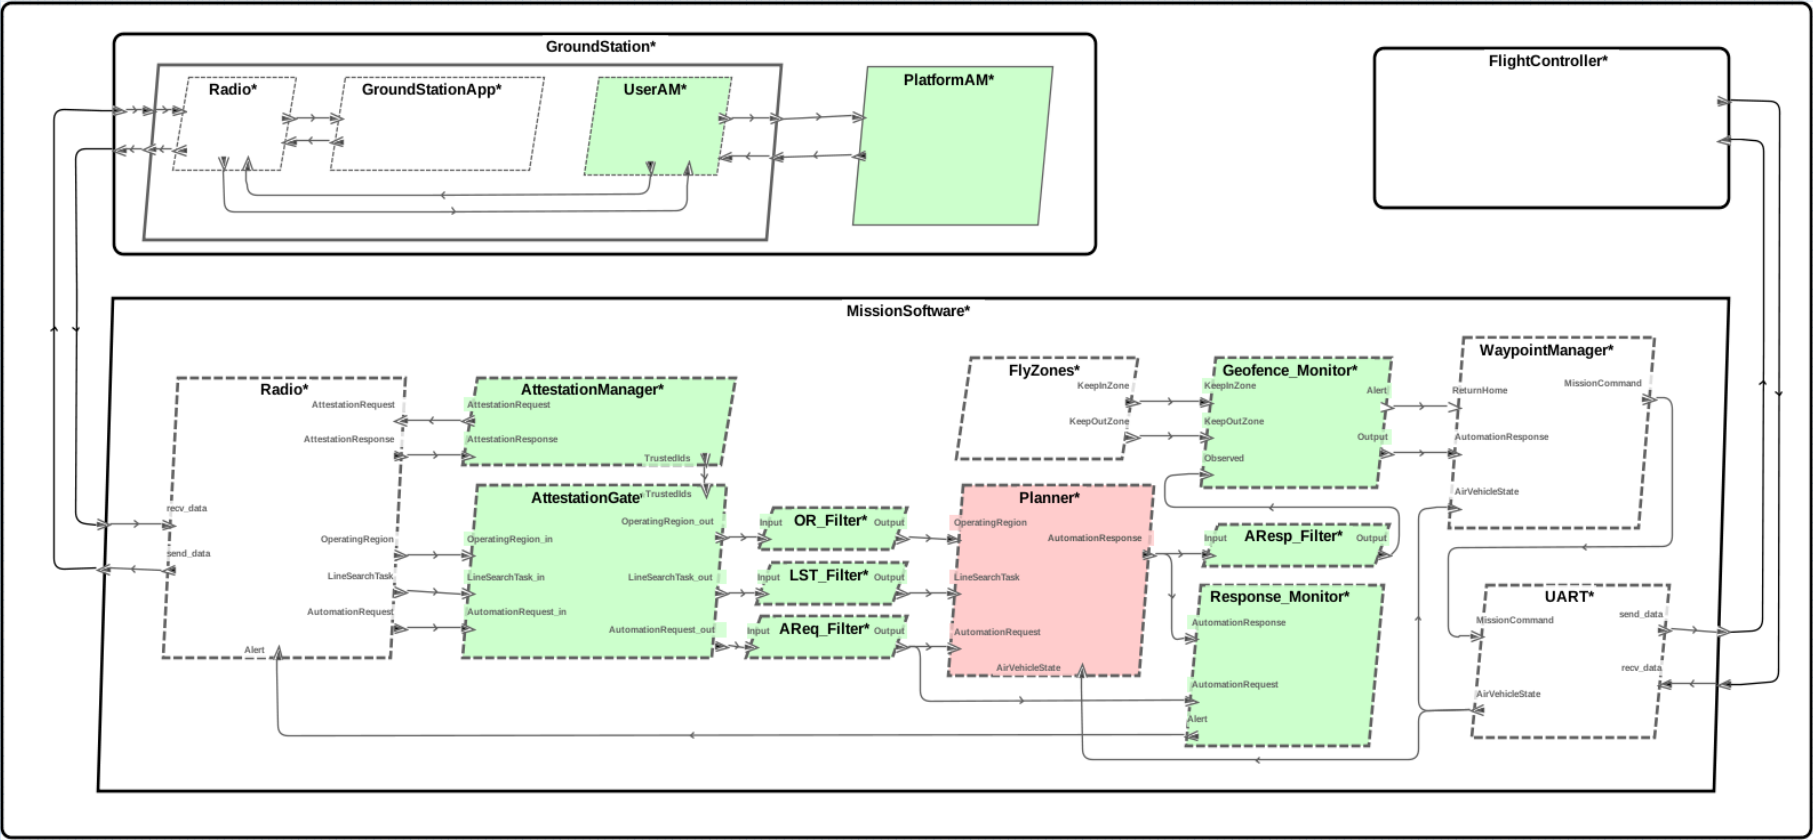
\includegraphics[width=2\columnwidth]{./figs/sw-hardened.png}
  \end{center}
	\caption{Cyber-resilient software architecture for UAV surveillance system.} 
	\label{fig:sw-hardened} 
\end{figure*}

\figref{fig:sw-hardened} is a model-based design in the AADL OSATE tool of a cyber-hardened software system for an autonomous UAV for surveillance.
The original \emph{unhardened system} consists of four components: the radio to communicate with a remote ground
station (\emph{Radio}), mission planning automation (\emph{UxAS}), waypoint metering (\emph{WaypointManager}), and a UART to talk to the flight controller (\emph{UART}).

\briefcase\ integrates four key formal methods in the model-based engineering workflow: assume-guarantee verification (\agree), synthesis of high-assurance components (\splat), synthesis of inter-component communication (\hamr), and the \selFour\ verified microkernel.
Each component in the unhardened system, and the interface for the top-level software component, is formally specified with an AGREE contract stating assumptions on inputs and guarantees on outputs under the assumptions.
\agree\ proves the unhardened implementation obeys the composition of these contracts. 

Cyber-threat analysis (GearCASE and DCRYPPS) identifies the ground station and the planning automation services as primary cyber threats to the system.
Seven new cyber requirements are added to the unhardened system that require ground station certification, message integrity, and monitoring.
The existing contracts in the unhardened system are strengthened to reflect these new requirements.
\agree\ proves the unhardened system under these contracts fails verification. 

Design engineers use \briefcase\ to transform the unhardened system to that in \figref{fig:sw-hardened} by inserting high-assurance components. 
\emph{Attestation} proves the identity of trusted ground stations (\emph{AttestationManager}) while the \emph{gate} only passes messages from trusted sources (\emph{AttestationGate}).
\emph{Filters} only pass well-formed messages (\emph{OR\_Filter}, \emph{LST\_Filter}, \emph{AReg\_Filter}, and \emph{AResl\_Filter}).
\emph{Monitors} alert to suspicious behavior such as missions that enter keep-out zones or leave keep-in zones (\emph{Geofence\_Monitor}) or unrequested missions from automation (\emph{Response\_Monitor}).
The interface behavior of these high-assurance components, with the exception of attestation, is specified with assume-guarantee contracts (e.g., a filter makes no assumptions on input and only passes input that is well-formed).
\agree\ proves the hardened system ensures the added cyber requirements.

The \selFour\ target platform requires a static schedule that is provided in the model.
A transformation on the \agree\ contracts incorporates that schedule into the verification model.
\agree\ proves the scheduled hardened system also ensures cyber requirements.
The model is further refined to move the attestation and mission planning services into separate virtual machines inside the microkernel.

\resolint\ certifies the hardened model is ready for synthesis.
\splat\ synthesizes high-assurance components from their \agree\ contracts to the target platform.
It includes proof certificates that the binaries have assumptions that are no stronger than those on the original contracts and guarantees that are no weaker than those on the original contracts (e.g., safe substitution).
\hamr\ synthesizes all the inter-component communication primitives from the AADL model.
That synthesis includes a proof certificate that the resulting communication channels defined in \selFour\ are only those defined in the AADL model.

\resolute\ builds an assurance case for the entire system.
That assurance case includes evidences for every requirement including proof certificates from \agree, \splat, and \hamr.
